%
% File emnlp2020.tex
%
%% Based on the style files for ACL 2020, which were
%% Based on the style files for ACL 2018, NAACL 2018/19, which were
%% Based on the style files for ACL-2015, with some improvements
%%  taken from the NAACL-2016 style
%% Based on the style files for ACL-2014, which were, in turn,
%% based on ACL-2013, ACL-2012, ACL-2011, ACL-2010, ACL-IJCNLP-2009,
%% EACL-2009, IJCNLP-2008...
%% Based on the style files for EACL 2006 by 
%%e.agirre@ehu.es or Sergi.Balari@uab.es
%% and that of ACL 08 by Joakim Nivre and Noah Smith

\documentclass[11pt,a4paper]{article}
\usepackage[hyperref]{emnlp2020}
\usepackage{times}
\usepackage{latexsym}
\renewcommand{\UrlFont}{\ttfamily\small}

%\aclfinalcopy

\special{papersize=210mm,297mm}

% This is not strictly necessary, and may be commented out,
% but it will improve the layout of the manuscript,
% and will typically save some space.
\usepackage{microtype}
\usepackage{graphicx}

%\aclfinalcopy % Uncomment this line for the final submission
%\def\aclpaperid{***} %  Enter the acl Paper ID here

%\setlength\titlebox{5cm}
% You can expand the titlebox if you need extra space
% to show all the authors. Please do not make the titlebox
% smaller than 5cm (the original size); we will check this
% in the camera-ready version and ask you to change it back.

\newcommand\BibTeX{B\textsc{ib}\TeX}

\def\PS#1{{\color{violet}PS: \it #1}}


\title{Creating Fiction Through De-summarization}

\author{Saad Obaid ul Islam \\
  MFF UK \\\And
  Patrícia Schmidtová \\
  MFF UK \\
  \texttt{schmidtova@ufal.mff.cuni.cz}
  }

\date{}

\begin{document}
\maketitle
\begin{abstract}
While story generation is on the rise, it seems that most of the effort is put into producing very short stories. We aim to change that by introducing an approach to gradually de-summarize a short prompt, such as a title, into a longer text. We present 3 models all of which beat the baseline language model in human evaluation. In addition to the models, we also present a new automatic metric based on the NLI task. This metric aims to assess the consistency of a text.
\end{abstract}


\section{Introduction}
In the last couple of years, there have been some promising breakthroughs in the field of open-ended story generation \citep{fan_hierarchical_2018, clark_neural_2018, ammanabrolu_guided_2019}. However, these works often focus on producing very short stories, such as those in the ROCstories dataset \citep{rocstories}. 

In our work, we are exploring a 'reverse summarization' approach in order to generate stories. In the summarization task, the input is the article/document and the output is a brief summary of that article/document. What we decided to do is to de-summarize, meaning we flip the inputs and outputs. The input is the summary (in our case, title of a movie/play) and output is the article (in our case, a story).  

While we are not yet ready to generate full-length plays, we have had success with producing longer stories. Since it is not possible to read every machine-generated output and evaluate it manually, we also present a new metric based on the NLI task which focuses on text consistency. 
\section{Dataset}
\label{sec:data}
Our dataset contained three types of data:
\begin{itemize}
    \item short stories (480 words on average)
    \item long stories (900 words on average)
    \item full-length scripts
\end{itemize}
We used two existing datasets: Wiki Movie Plots dataset \citep{wikidataset} which contains short summaries of movies from Wikipedia and Movie Plot Synopses with Tags dataset \citep{movieplotdataset} which contains short summaries of movies from both Wikipedia and IMDb. The rest of the data we used has been compiled during the work on the THEaiTRE project \citep{theaitre} and contains short and long theatre play summaries from Wikipedia, Sparknotes and various fan-sourced websites. This portion of data also contains the full-length scripts of movies and episodes of TV shows taken from fan-sourced script collections such as the IMSDb\footnote{https://imsdb.com/} or Forever Dreaming Transcripts.\footnote{https://transcripts.foreverdreaming.org/}

During the preprocessing phase, the data was cleared of duplicities, corresponding summaries were merged with the scripts, and the data was separated into a train and test split with a ratio 9:1. The absolute amounts of examples can be seen in Table \ref{tab:data}.

\begin{table}[]
    \centering
    \begin{tabular}{c|c}
    \textbf{Type of Data}  & \textbf{Examples}  \\\hline
    Short summaries     & $\sim$40K \\
    Long summaries & $\sim$1.5K \\
    Scripts & $\sim$1.6K
    \end{tabular}
    \caption{Amount of data}
    \label{tab:data}
\end{table}

\begin{figure}
    \centering
    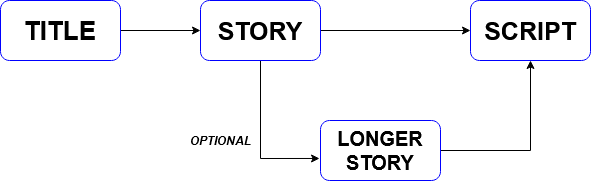
\includegraphics[width=0.47\textwidth]{flowchart.png}
    \caption{Hierarchical generation approach}
    \label{fig:flowchart}
\end{figure}

\section{Approach}
Language models are not yet capable of producing a full-length play by themselves \citep{theaitre} and often produce texts which are uninteresting and heavily repetitive \citep{see-etal-2019-massively}. Our goal was to develop a pipeline which would allow us to progressively generate longer texts without serious declines in coherence and consistency.

With this goal in mind, we present our hierarchical approach. As illustrated in Figure \ref{fig:flowchart}, we aim to break the generation down into a couple of steps:
\begin{enumerate}
    \item Produce a short story when given a story title.
    \item Optionally elaborate on the short story and turn it into a longer one.
    \item Separate the stories into sentences or other blocks
    \item Use the blocks to generate short scripts
    \item Concatenate the short scripts into a single script
\end{enumerate}
These steps are inspired by the data we have. We have alignments between all the proposed transitions, however the amount of aligned data containing scripts was not sufficient to make the model work. So far, we can present models involved in steps 1 and 2. Further dataset improvements will have to be made in order to successfully produce models which can generate scripts.



\section{Models}
\label{sec:models}

We fine-tune the following three models: 
\begin{itemize}
    \item GPT-2 \citep{radford2019language}  was developed by OpenAI for text generation. GPT-2 is a large transformer based model with 1.5 billion parameters. It generates synthetic text in response to the model being prompted with an arbitary input. 
    \item PEGASUS \citep{zhang2019PEGASUS} was developed by researchers at Google AI for abstractive summarization. It achieved state of the art performance on 12 summarization tasks.
    \item DistilBART \citep{distilbart} was developed by researchers at Facebook AI for practical use of large scare pre-trained transformers. They apply 'shrink and fine-tune' method to original BART \citep{bart2019} and PEGASUS.    
\end{itemize}



\section{Evaluation}
\label{sec:eval}
Since this work is one of the first in its kind, there are no established evaluation metrics and procedures yet.
For this reason, we use some well-established metrics (such as perplexity or ROUGE score), perform manual evaluation, and propose our own automatic metric based on the NLI task. We have used 500 examples generated from the test set in our automatic evaluation process.

\subsection{Supervised Metrics}
We use two automatic evaluation metrics; ROUGE score \citep{lin-2004-rouge} and BERTScore \citep{Zhang*2020BERTScore:}. We call them supervised, because both of them need a reference text. ROUGE measures n-gram precision, recall, and f-measure between candidate and reference text. It is presently mostly used for evaluating summarization systems. BERTScore measures the cosine similarity in contextual embeddings between candidate and reference text. It was proposed in 2020 as an improvement to previous automatic evaluation metrics for text generation. 

\paragraph{Results}

In Table \ref{tab:rouge} we can observe that GPT-2 performed considerably well compared to PEGASUS and DistilBART. This is a bit surprising since PEGASUS and DistilBART are Seq2Seq models so we hypothesized that they will be able to encode the prompts better. 

However, the problem with ROUGE score is that it is an n-gram matching based evaluation. So we also use BERTScore which captures the position and context of the word by computing cosine similarity using contextual word embeddings. In Table \ref{tab:bertscore} we can see that the GPT-2 is again performing better than DistilBART and PEGASUS but only by a few decimals. This indicates that all three of them were able to generate semantically correct sentences

\begin{table}[] % Apparently the asterisk makes it centered (instead of being in one column)
    \centering
    \begin{tabular}{|c|c|c|c|} % Here you need to declare how many columns you want to have. The c means that the content is centered. There is also r and l for right and left alignment
    \hline % This is how horizontal lines are added, you can put them anywhere  
    \textbf{Model}   & \textbf{Precision} & \textbf{Recall} & \textbf{F-measure}  \\\hline
      GPT-2   & 26.65 & 30.83 & 22.12 \\
      PEGASUS & 26.70 & 6.04 & 8.35 \\
      DistilBART & 32.14 & 13.30 & 15.44 \\
    \hline
    \end{tabular}
    \caption{ROUGE uni-gram scores}
    \label{tab:rouge}
    \begin{tabular}{|c|c|c|c|} % Here you need to declare how many columns you want to have. The c means that the content is centered. There is also r and l for right and left alignment
    \hline % This is how horizontal lines are added, you can put them anywhere  
    \textbf{Model}   & \textbf{Precision} & \textbf{Recall} & \textbf{F-measure}  \\\hline
      GPT-2   & 81.84 & 81.80 & 81.80 \\
      PEGASUS & 82.54 & 80.13 & 81.29 \\
      DistilBART & 82.06 & 80.99 & 81.51 \\
    \hline
    \end{tabular}
    \caption{BERTScore}
    \label{tab:bertscore}
\end{table}


\subsection{Unsupervised Metrics}
Since we would like to be able to evaluate open-ended story generation with potentially no reference text, it is desirable to suggest metrics which do not require it.
All of the average values of the metrics and characteristics listed below can be found in Table \ref{tab:automatic}. By no means do we consider the following list of metrics to be exhaustive.

\paragraph{Sentence length}
We have elected to observe sentence length, because texts containing sentences that are too long tend to be more difficult to read. On the other hand, sentences are too short increase the monotonicity of a text, making it duller. In order to get a better idea about what values we should aim for, we also ran the evaluation on the test set which contains human-written stories. In Table \ref{tab:automatic} we can see that all models are very close to the average human sentence length with DistilBART being the closest.

\paragraph{Story length}
As we mentioned in the introduction, most of the previous work focuses on short stories that are around 5 sentences long. Since our goal is to generate longer texts, it makes sense to try to capture just how much longer they are. Of course, this can be influenced via a decoding parameter, but our models can also choose to end generating before reaching the maximum length. We report the length in sentences and words. Table \ref{tab:automatic} shows that GPT-2 is capable of writing the longest summaries and therefore is the closest to the golden lengths we wish to achieve.

\paragraph{Perplexity}
Perplexity is a standard metric for any natural language generation task. If it is too low, it can indicate that the text is repetitive or uninteresting. In the opposite case, when the perplexity is unusually high, it could potentially mean that the text does not adhere to a proper grammatical structure. Looking at Table \ref{tab:automatic}, we can find it strange that stories generated by GPT-2 have a higher perplexity on average. This could mean that GPT-2 is producing unlikely and/or original stories. However, this number alone is not enough to determine whether that hypothesis is true. It is necessery to assess the behavior of the model using human evaluation.


\begin{table*}[]
    \centering
    \begin{tabular}{|c|c|c|c|c|}
    \hline
    \textbf{Model}  & \textbf{Length} & \textbf{Sentences} & \textbf{Words} & \textbf{Perplexity} \\\hline
    Test set & 21  & 482 & 25 & 2.41 \\
    GPT-2 & 19 & 377 & 20 & 3.15 \\
    PEGASUS & 18 & 53 & 3 & 1.31 \\
    DistilBART & 20 & 107 & 6 & 1.54 \\
    \hline
    \end{tabular}
    \caption{The average values of automatic metrics}
    \label{tab:automatic}
\end{table*}

\subsection{NLI-based Consistency Metric}
\label{sec:nli}
The natural language inference (NLI) task is to determine whether a given sentence is entailed in, neutral to, or in contradiction with a piece of text.
This is useful for us, because we want to avoid inconsistencies -- contradictions.
At the same time, entailment is also not preferable, because it can indicate repetition.
Essentially, we are interested in how neutral a given sentence is in relation to the preceding text.
This neutrality is computed by using the roberta-large-mnli model by \cite{liu2019roberta}.

Instead of just approaching this task as a classification, we apply softmax over the logits given by the model in order to obtain a distribution of the categories.
Then we take the probability of the 'neutral' category as the basis for our score.
We are using this approach instead of counting the occurence of classified categories, because we found that on our data, the model almost never openly states that a sentence is a contradiction or an entailment -- neutral is always prominent.
However, the changes in distribution usually do reflect the requested result.

In order to make the metric resistant to reasonable changes in the length of evaluated text, we propose to measure the average neutrality per added sentence.
The second sentence is compared with the first, the third with the first two, and so on.
Once the chunk of preceding text became too long to fit into the model, we truncated it by removing entire sentences from the beginning.

\begin{table}[]
    \centering
    \begin{tabular}{|c|c|c|}
    \hline
    \textbf{Model} & \textbf{NLI-Score} & \textbf{Std}  \\\hline
    Test set &  0.73  & 0.16  \\
    GPT-2 &  0.68  &  0.1 \\
    PEGASUS &  0.68  & 0.16 \\
    DistilBART & 0.67 & 0.13 \\
    \hline
    \end{tabular}
    \caption{Average NLI-Score and the standard deviation}
    \label{tab:nli}
\end{table}

\subsubsection{Results of the NLI-Score}


We can see the results of this evaluation in Table \ref{tab:nli}. According to the metric, each of our models performs on a similar level than the human-written stories. However, it is necessary to point out that in case of DistilBART and PEGASUS, we found that the models sometimes produced the same story many times -- regardless of the title. These stories scored pretty high in our similarity metric and therefore are pushing the average values up.

It is also important to look back at Table \ref{tab:automatic} and realize that DistilBART and PEGASUS produced much shorter stories on average. Naturally, it is easier not to run into any contradictions or entailments when the story is very short.

\subsubsection{Limitations of the metric}
As we can see, even the human-written stories do not score as high as we had originally expected. This can be due to two reasons:

\paragraph{Error in NLI classification}
The model which classifies the sentences into the NLI categories is not a 100\% accurate. It is quite possible that it makes mistakes, especially if a contradiction is very subtle. 

\paragraph{Is neutrality what we want?}
We have described our reasons for wanting the generated sentences to be as neutral as possible to the previous ones. However, this might not be the optimal approach. Perhaps plot twists are meant to contain contradictions, or some level of entailment can improve the quality of the story.

\subsubsection{Potential usage}
In a human-in-the-loop scenario, this metric can be used for filtering out stories that are objectively not consistent. We would recommend setting the threshold somewhere between 0.3 - 0.5, based on the individual's preference.

\subsection{Manual Evaluation}
Since evaluating almost any natural language generation task is very subjective and cannot yet be captured by automatic metrics, it is necessary to perform manual evaluation. Apart from our fine-tuned models described in Section \ref{sec:models}, the manual evaluation also featured a vanilla GPT-2-medium as the baseline.
We carried out two manual evaluation procedures:

\subsubsection{Relative ranking}
The annotators were asked to look at 3 stories at a time. Their task was to order them from the best to the worst according to their own subjective judgement with no further instructions. In total, we had 6 annotators looking at 12 stories in 4 comparisons. 

\begin{table}[]
    \centering
    \begin{tabular}{|c|c|c|c|}
    \hline
    \textbf{Model} &\textbf{1st} &\textbf{2nd} & \textbf{3rd} \\\hline
    Baseline & 4 & 6 & 8 \\
    GPT-2 & 5 & 9 & 4 \\
    PEGASUS & 8 & 5 & 5 \\
    DistilBART & 7 & 4 & 7 \\\hline
    \end{tabular}
    \caption{The relative ranking results}
    \label{tab:ranking}
\end{table}

As can be seen in Table \ref{tab:ranking}, every one of our models outperformed the baseline in this task. GPT-2 was most frequently the "middle option" and was considered to be the worst the least amount of times. According to our annotators, the best stories were written by Pegasus. An interesting phenomenon occured while evaluating DistilBART - there were 2 annotators who selected DistilBART as their top choice whenever it was present in the comparison.


\subsubsection{Absolute scoring}
The annotators were shown one story at a time and were asked to evaluate it in terms of:
\begin{itemize}
    \item Coherence -- Is the text coherent?
    \item Consistency -- Are the characters consistent?
    \item Originality -- Is the text original and/or interesting?
    \item Title Relevance -- Is the title relevant to the story?
    \item Overall Impression -- Did you enjoy reading this text?
\end{itemize}

Each of the attributes was rated on a 5-point scale with 1 being the worst, and 5 being the best.

\begin{table*}[]
    \centering
    \begin{tabular}{|c|c|c|c|c|c|}
    \hline
    \textbf{Model} &\textbf{Coherence} &\textbf{Consistency} & \textbf{Originality} & \textbf{Relevance} &\textbf{Overall Impression} \\\hline
    Baseline & 2.7 & 2.8 & 2.6 & 2.7 & 2.6 \\
    GPT-2 & 3 & 3.1 & 3.1 & 2.6 & 3.2 \\
    PEGASUS & 2.8 & 2.8 & 3 & 2.1 & 2.8 \\
    DistilBART & 1.9 & 2 & 3.2 & 2 & 2.9 \\
    \hline
    \end{tabular}
    \caption{The average absolute scores}
    \label{tab:absolute}
\end{table*}

In this evaluation task, GPT-2 proved to be the best all-around model. It only slightly under-performs the baseline in the title relevance ranking. We hypothesize that this is the case, because our models were trained on data which included more abstract relations between the title and the story. The baseline then uses the titles more literally than our models.


\section{Conclusion}
We have presented an approach to generate longer texts which are still conditioned on an input prompt -- in our case the title. By gradually de-summarizing the title, we hope to eventually arrive at a computer generated full-length script.

We have trained and evaluated 3 separate models. Based on the evaluation, we consider our fine-tuned GPT-2 to be the most useful model for our continued attempts to generate a theatre play.

We have also presented a new metric for natural language generation based on the NLI task. We are also hoping to improve a possible human-in-the-loop scenario by using this metric as a filter.

As future work, we are hoping to devise a similar system for evaluating even longer stories. Moreover, we are hoping to bridge the gap between the stories we have now and the scripts they could become.


\bibliographystyle{acl_natbib}
\bibliography{emnlp2020}

\appendix

\section{Samples of Generated Stories}
\label{sec:appendix}
\subsection{GPT-2}
\paragraph{The Haunted House Mystery}
The film is set in the late 19th century, in the small town of Fairfield, New Hampshire, where the story is told. The story begins with a young woman named Susan, who is haunted by the ghost of her deceased mother, who died in a car accident. Susan and her family are forced to move into a dilapidated house on the outskirts of town.
Susan's mother died in an automobile accident, leaving her with no memory of what happened to her mother. Susan begins to remember the events of her mother's death, including the car accident that killed her mother, and the death of her stepfather, who was also killed in the accident. She begins to suspect that the ghost may be responsible for the deaths of her father and stepmother.


\subsection{DistilBART}
\paragraph{An empty bag and a dead Eve in the Tunnel}
The Tunnel Troll has been searching for a new identity since it was pulled over by the racist, homophobic, and sexist Sheriff Dollard. He discovers the truth behind the infamous "drag princess" incident in the tunnel.
While searching for the new identity of the drag queen, Dollard is ridiculed for her actions by her colleagues, who believe she was a drag queen.

\subsection{Pegasus}
\paragraph{Three and Two is Five}
During the reign of Queen Elizabeth I, England is concerned by the impending arrival of the Spanish Armada. In 1588, relations between Spain and England are at breaking point. With the support of Queen Victoria, English privateers such as Sir Francis Drake regularly capture Spanish merchantmen bringing gold from the New World. Elizabeth's chief advisers are the Lord Treasurer, Lord Burleigh, and her longtime admirer, Robert Dudley, Earl of Leicester. Burleigh's 18-year-old granddaughter Cynthia is one of Elizabeth' three widows, and the ageing queen is plagued by guilt over the girl's alleged involvement in prostitution.



\end{document}
